\section{Objectives and Activities}

The project targets to evaluate the scalability of the two kind of compositions explained above. To make this evaluation, we first needed a composition to evaluate. Thus we designed a synthetical orchestration in witch each partner is another synthetical orchestration, recursively, the second's partners are also orchestrated services, until the last specific composition. The topology generated from this design is a tree, each node (first kind of orchestrated service) has a pre-defined number of children. The depth of the tree is also predefined. The message received in the root node is propagated through it's children until it reaches the leaf node (the second kind of service on the process). When the leaf node receives the message, it starts the travel back to the root, which replies to the client. A simple example with 3 children per node and depth of 2 is shown in Figure \ref{synthetical-example}.

\begin{figure}[htb]
	\centering
	\includegraphics[width=\textwidth]{images/synthetical-example}
	\caption{Example of a composition with 3 children per node and depth of 2. With it's flow of messages}
	\label{synthetical-example}
\end{figure}
\newpage

This tree is a choreography of orchestrated services: each node and it's children are the orchestration and the entire process is a choreography.

\subsection{Composition Generator}
To generate the tree structure described above, we first developed ``hardcoded'' orchestrations with NetBeans to simulate the desired tree. When we accomplished this first task, we created a Ruby script which generated the tree and, also, for each node of the tree, a set of WSDL and BPEL files corresponding to the service of that node.

Later, we needed an automate way to deploy all those services on different machines, so we attached some more code to the Ruby script to allocate instances of Amazon EC2 for each node of the tree. In this moment the code was starting to get ugly. It was time for refactoring.

After spending some time to make the code more readable, we decided to develop the deploy of the process in the instances of EC2. But NetBeans, used until this point to run the process generated, was not able to run properly from the command-line shell, which is the only native interface with EC2 instances. After some research upon open source engines, we discovered PEtALS ESB, which has the simplest install and setup process among all the servers studied; this was the most essential feature to build the automated process.

Currently, the script generates the tree, instantiates virtual machines on Amazon EC2, creates the compositions, configures each instance to become a node of the PEtALS Bus, starts the PEtALS server in each node, and deploys the services on the ESB. This process is parallelized for each node, and the steps of the process can be followed in the shell's standard output, as shown in Figure \ref{generation-output}.

\begin{figure}[htb]
	\centering
	\includegraphics[trim= 10mm 0mm 10mm 0mm, clip, width=\textwidth]{images/generation-output}
	\caption{Example output from running the generator script for a tree with depth of 1 and 10 children per node}
	\label{generation-output}
\end{figure}

When it is finished, the generator outputs the host of the process (\emph{Public DNS} of Root Node), from which port it is reachable, the path to the service, and the ID of this root node (to compose the SOAP messages).

\subsection{Message Sender}

To evaluate the responses of the synthetical compositions, we needed another Ruby script to send messages of sizes $s$ and with a frequency of $f$ messages per second.

Given the fact that the connection with the Cloud is very unstable, we added a third parameter to define how many times the batch of messages will be sent, so when there is a lot of traffic on the network, any extraordinary case will not be representative on the overall average. During execution, the script shows four numbers for each batch of messages sent, they represent (in order they appear):
\begin{itemize} 
	\item[user] is the time spent (in seconds) with the execution of actions of the script, for example calling a class method
	\item[system] is the time spent (in seconds) with system calls, for example creating a \emph{fork}
	\item[total] is the sum of \emph{user} and \emph{system} times
	\item[real] is how long passed (in seconds) from the task begins until its end
\end{itemize}

An example of it's execution is shown in Figure \ref{send-msg-output}.


\begin{figure}[htb]
	\centering
	\includegraphics[width=0.8\textwidth]{images/send-msg-output}
	\caption{Example output from running the send message script with $S = 1$, $F = 1$, $BatchSize = 10$}
	\label{send-msg-output}
\end{figure}
